\documentclass[letterpaper]{article} % DO NOT CHANGE THIS
\usepackage[submission]{aaai2027}  % DO NOT CHANGE THIS
\usepackage[hyphens]{url}  % DO NOT CHANGE THIS
\usepackage{graphicx} % DO NOT CHANGE THIS
\urlstyle{rm} % DO NOT CHANGE THIS
\def\UrlFont{\rm}  % DO NOT CHANGE THIS
\usepackage{natbib}  % DO NOT CHANGE THIS AND DO NOT ADD ANY OPTIONS TO IT
\usepackage{caption} % DO NOT CHANGE THIS AND DO NOT ADD ANY OPTIONS TO IT
\frenchspacing  % DO NOT CHANGE THIS
\usepackage{algorithm}
\usepackage{algorithmic}
\usepackage{booktabs}
\usepackage{amsmath}
\usepackage{amsthm}
\usepackage{tikz}
\usetikzlibrary{positioning,arrows.meta}
\pdfinfo{
/TemplateVersion (2027.1)
}
% generated by make_numbers.py -- do not edit
\newcommand{\Classification}{CONDITIONAL_GO}
\newcommand{\CritCFive}{True}
\newcommand{\CritCFour}{True}
\newcommand{\CritCOne}{True}
\newcommand{\CritCSix}{False}
\newcommand{\CritCThree}{inconclusive}
\newcommand{\CritCTwo}{True}
\newcommand{\Critvalidity}{True}
\newcommand{\DevOnecritexpandVsBFiveCI}{[-0.0245, -0.0126]}
\newcommand{\DevOnecritexpandVsBFiveHolm}{3.1\cdot10^{-5}}
\newcommand{\DevOnecritexpandVsBFiveRel}{44.5}
\newcommand{\DevOnecritexpandVsBFiveSign}{-}
\newcommand{\DevOnecritexpandVsBFiveWL}{20/0}
\newcommand{\DevOnecritexpandVsBZeroCI}{[-0.0140, -0.0057]}
\newcommand{\DevOnecritexpandVsBZeroHolm}{6.0\cdot10^{-4}}
\newcommand{\DevOnecritexpandVsBZeroRel}{29.4}
\newcommand{\DevOnecritexpandVsBZeroSign}{-}
\newcommand{\DevOnecritexpandVsBZeroWL}{19/1}
\newcommand{\DevOnecritexpandVstimewindowCI}{[-0.0025, +0.0046]}
\newcommand{\DevOnecritexpandVstimewindowHolm}{1.00}
\newcommand{\DevOnecritexpandVstimewindowRel}{4.9}
\newcommand{\DevOnecritexpandVstimewindowSign}{+}
\newcommand{\DevOnecritexpandVstimewindowWL}{10/10}
\newcommand{\FigTwoOneFiveCritAt}{1.0}
\newcommand{\FigTwoOneFiveSrAt}{1.3}
\newcommand{\FigTwoOneFiveTwAt}{1.2}
\newcommand{\FigTwoTwoZeroCritAt}{1.7}
\newcommand{\FigTwoTwoZeroSrAt}{2.8}
\newcommand{\FigTwoTwoZeroTwAt}{2.0}
\newcommand{\MTwoRoundCritFeas}{376}
\newcommand{\MTwoRoundCritInfeas}{7988}
\newcommand{\MTwoRoundCritN}{82.4}
\newcommand{\MTwoRoundCritSolverS}{0.056}
\newcommand{\MTwoRoundTwFeas}{901}
\newcommand{\MTwoRoundTwInfeas}{7289}
\newcommand{\MTwoRoundTwN}{82.3}
\newcommand{\MTwoRoundTwSolverS}{0.080}
\newcommand{\MTwoRoundTwVsCritPct}{43}
\newcommand{\MechTwoArrivalN}{40}
\newcommand{\MechTwoArrivalRel}{8.9}
\newcommand{\MechTwoArrivalWL}{13/27}
\newcommand{\MechTwoCancellationN}{38}
\newcommand{\MechTwoCancellationRel}{18.5}
\newcommand{\MechTwoCancellationWL}{9/29}
\newcommand{\MechTwoDurationN}{38}
\newcommand{\MechTwoDurationRel}{13.3}
\newcommand{\MechTwoDurationWL}{12/26}
\newcommand{\MechTwoOutageN}{31}
\newcommand{\MechTwoOutageRel}{9.8}
\newcommand{\MechTwoOutageWL}{11/20}
\newcommand{\OracleCpsatCases}{1{,}000}
\newcommand{\OracleEnumCases}{2{,}000}
\newcommand{\RoundCritRate}{66}
\newcommand{\RoundTimewinRate}{50}
\newcommand{\RoundsUOneArrivalCrit}{3.15}
\newcommand{\RoundsUOneArrivalTw}{2.02}
\newcommand{\RoundsUOneCancelCrit}{2.40}
\newcommand{\RoundsUOneCancelTw}{1.85}
\newcommand{\RoundsUOneDurationCrit}{2.91}
\newcommand{\RoundsUOneDurationTw}{2.06}
\newcommand{\RoundsUOneOutageCrit}{2.95}
\newcommand{\RoundsUOneOutageTw}{1.88}
\newcommand{\UEightBTwocritVsBSixporthintCI}{[-0.0238, -0.0142]}
\newcommand{\UEightBTwocritVsBSixporthintHolm}{5.7\cdot10^{-6}}
\newcommand{\UEightBTwocritVsBSixporthintRel}{43.0}
\newcommand{\UEightBTwocritVsBSixporthintSign}{-}
\newcommand{\UEightBTwocritVsBSixporthintWL}{20/0}
\newcommand{\UEightBTwocritVsBThreetimewinCI}{[-0.0059, -0.0001]}
\newcommand{\UEightBTwocritVsBThreetimewinHolm}{0.12}
\newcommand{\UEightBTwocritVsBThreetimewinRel}{9.5}
\newcommand{\UEightBTwocritVsBThreetimewinSign}{-}
\newcommand{\UEightBTwocritVsBThreetimewinWL}{14/6}
\newcommand{\UEightBTwocritVsBZeroiaipCI}{[-0.0090, -0.0030]}
\newcommand{\UEightBTwocritVsBZeroiaipHolm}{0.024}
\newcommand{\UEightBTwocritVsBZeroiaipRel}{18.8}
\newcommand{\UEightBTwocritVsBZeroiaipSign}{-}
\newcommand{\UEightBTwocritVsBZeroiaipWL}{16/4}
\newcommand{\UEightMeanBSixporthint}{.0441}
\newcommand{\UEightMeanBThreetimewin}{.0278}
\newcommand{\UEightMeanBTwocrit}{.0252}
\newcommand{\UEightMeanBZeroiaip}{.0310}
\newcommand{\UEightN}{20}
\newcommand{\UEightRecords}{4{,}400}
\newcommand{\UFiveBTwocritVsBSixporthintCI}{[-0.0162, -0.0090]}
\newcommand{\UFiveBTwocritVsBSixporthintHolm}{5.7\cdot10^{-6}}
\newcommand{\UFiveBTwocritVsBSixporthintRel}{42.5}
\newcommand{\UFiveBTwocritVsBSixporthintSign}{-}
\newcommand{\UFiveBTwocritVsBSixporthintWL}{20/0}
\newcommand{\UFiveBTwocritVsBThreetimewinCI}{[-0.0029, +0.0003]}
\newcommand{\UFiveBTwocritVsBThreetimewinHolm}{0.26}
\newcommand{\UFiveBTwocritVsBThreetimewinRel}{7.0}
\newcommand{\UFiveBTwocritVsBThreetimewinSign}{-}
\newcommand{\UFiveBTwocritVsBThreetimewinWL}{13/7}
\newcommand{\UFiveBTwocritVsBZeroiaipCI}{[-0.0060, -0.0022]}
\newcommand{\UFiveBTwocritVsBZeroiaipHolm}{0.005}
\newcommand{\UFiveBTwocritVsBZeroiaipRel}{19.2}
\newcommand{\UFiveBTwocritVsBZeroiaipSign}{-}
\newcommand{\UFiveBTwocritVsBZeroiaipWL}{17/3}
\newcommand{\UFiveMeanBSixporthint}{.0293}
\newcommand{\UFiveMeanBThreetimewin}{.0181}
\newcommand{\UFiveMeanBTwocrit}{.0168}
\newcommand{\UFiveMeanBZeroiaip}{.0209}
\newcommand{\UFiveN}{20}
\newcommand{\UFiveRecords}{2{,}640}
\newcommand{\UFourBTwocritVsBSixporthintCI}{[-0.0147, -0.0057]}
\newcommand{\UFourBTwocritVsBSixporthintHolm}{0.002}
\newcommand{\UFourBTwocritVsBSixporthintRel}{20.7}
\newcommand{\UFourBTwocritVsBSixporthintSign}{-}
\newcommand{\UFourBTwocritVsBSixporthintWL}{31/9}
\newcommand{\UFourBTwocritVsBThreetimewinCI}{[-0.0035, +0.0025]}
\newcommand{\UFourBTwocritVsBThreetimewinHolm}{0.86}
\newcommand{\UFourBTwocritVsBThreetimewinRel}{1.3}
\newcommand{\UFourBTwocritVsBThreetimewinSign}{-}
\newcommand{\UFourBTwocritVsBThreetimewinWL}{22/18}
\newcommand{\UFourBTwocritVsBZeroiaipCI}{[-0.0059, +0.0007]}
\newcommand{\UFourBTwocritVsBZeroiaipHolm}{0.86}
\newcommand{\UFourBTwocritVsBZeroiaipRel}{6.2}
\newcommand{\UFourBTwocritVsBZeroiaipSign}{-}
\newcommand{\UFourBTwocritVsBZeroiaipWL}{23/17}
\newcommand{\UFourMeanBSixporthint}{.0495}
\newcommand{\UFourMeanBThreetimewin}{.0397}
\newcommand{\UFourMeanBTwocrit}{.0392}
\newcommand{\UFourMeanBZeroiaip}{.0418}
\newcommand{\UFourN}{40}
\newcommand{\UFourRecords}{8{,}800}
\newcommand{\UNineBTwocritVsBSixporthintCI}{[-0.0402, -0.0285]}
\newcommand{\UNineBTwocritVsBSixporthintHolm}{3.5\cdot10^{-10}}
\newcommand{\UNineBTwocritVsBSixporthintRel}{53.2}
\newcommand{\UNineBTwocritVsBSixporthintSign}{-}
\newcommand{\UNineBTwocritVsBSixporthintWL}{34/0}
\newcommand{\UNineBTwocritVsBThreetimewinCI}{[-0.0057, +0.0014]}
\newcommand{\UNineBTwocritVsBThreetimewinHolm}{0.23}
\newcommand{\UNineBTwocritVsBThreetimewinRel}{6.9}
\newcommand{\UNineBTwocritVsBThreetimewinSign}{-}
\newcommand{\UNineBTwocritVsBThreetimewinWL}{21/13}
\newcommand{\UNineBTwocritVsBZeroiaipCI}{[-0.0193, -0.0093]}
\newcommand{\UNineBTwocritVsBZeroiaipHolm}{8.1\cdot10^{-9}}
\newcommand{\UNineBTwocritVsBZeroiaipRel}{31.5}
\newcommand{\UNineBTwocritVsBZeroiaipSign}{-}
\newcommand{\UNineBTwocritVsBZeroiaipWL}{33/1}
\newcommand{\UNineMeanBSixporthint}{.0641}
\newcommand{\UNineMeanBThreetimewin}{.0322}
\newcommand{\UNineMeanBTwocrit}{.0300}
\newcommand{\UNineMeanBZeroiaip}{.0438}
\newcommand{\UNineN}{34}
\newcommand{\UNineRecords}{7{,}480}
\newcommand{\UOneBOnerandomVsBZeroiaipCI}{[-0.0024, +0.0006]}
\newcommand{\UOneBOnerandomVsBZeroiaipHolm}{0.87}
\newcommand{\UOneBOnerandomVsBZeroiaipRel}{2.5}
\newcommand{\UOneBOnerandomVsBZeroiaipSign}{-}
\newcommand{\UOneBOnerandomVsBZeroiaipWL}{21/19}
\newcommand{\UOneBThreetimewinVsBZeroiaipCI}{[-0.0087, -0.0031]}
\newcommand{\UOneBThreetimewinVsBZeroiaipHolm}{5.5\cdot10^{-4}}
\newcommand{\UOneBThreetimewinVsBZeroiaipRel}{17.4}
\newcommand{\UOneBThreetimewinVsBZeroiaipSign}{-}
\newcommand{\UOneBThreetimewinVsBZeroiaipWL}{32/8}
\newcommand{\UOneBTwocritVsBFivenativeOnewCI}{[-0.0239, -0.0162]}
\newcommand{\UOneBTwocritVsBFivenativeOnewHolm}{1.5\cdot10^{-11}}
\newcommand{\UOneBTwocritVsBFivenativeOnewRel}{43.8}
\newcommand{\UOneBTwocritVsBFivenativeOnewSign}{-}
\newcommand{\UOneBTwocritVsBFivenativeOnewWL}{40/0}
\newcommand{\UOneBTwocritVsBFourprecCI}{[-0.0109, -0.0060]}
\newcommand{\UOneBTwocritVsBFourprecHolm}{3.3\cdot10^{-5}}
\newcommand{\UOneBTwocritVsBFourprecRel}{24.5}
\newcommand{\UOneBTwocritVsBFourprecSign}{-}
\newcommand{\UOneBTwocritVsBFourprecWL}{34/6}
\newcommand{\UOneBTwocritVsBOnerandomCI}{[-0.0088, -0.0046]}
\newcommand{\UOneBTwocritVsBOnerandomHolm}{8.3\cdot10^{-6}}
\newcommand{\UOneBTwocritVsBOnerandomRel}{20.4}
\newcommand{\UOneBTwocritVsBOnerandomSign}{-}
\newcommand{\UOneBTwocritVsBOnerandomWL}{35/5}
\newcommand{\UOneBTwocritVsBSixporthintCI}{[-0.0230, -0.0154]}
\newcommand{\UOneBTwocritVsBSixporthintHolm}{1.5\cdot10^{-11}}
\newcommand{\UOneBTwocritVsBSixporthintRel}{42.7}
\newcommand{\UOneBTwocritVsBSixporthintSign}{-}
\newcommand{\UOneBTwocritVsBSixporthintWL}{40/0}
\newcommand{\UOneBTwocritVsBThreetimewinCI}{[-0.0036, +0.0002]}
\newcommand{\UOneBTwocritVsBThreetimewinHolm}{0.16}
\newcommand{\UOneBTwocritVsBThreetimewinRel}{6.1}
\newcommand{\UOneBTwocritVsBThreetimewinSign}{-}
\newcommand{\UOneBTwocritVsBThreetimewinWL}{26/14}
\newcommand{\UOneBTwocritVsBZeroiaipCI}{[-0.0097, -0.0053]}
\newcommand{\UOneBTwocritVsBZeroiaipHolm}{8.3\cdot10^{-6}}
\newcommand{\UOneBTwocritVsBZeroiaipRel}{22.4}
\newcommand{\UOneBTwocritVsBZeroiaipSign}{-}
\newcommand{\UOneBTwocritVsBZeroiaipWL}{35/5}
\newcommand{\UOneMeanBFivenativeOnew}{.0456}
\newcommand{\UOneMeanBFourprec}{.0340}
\newcommand{\UOneMeanBOnerandom}{.0322}
\newcommand{\UOneMeanBSixporthint}{.0447}
\newcommand{\UOneMeanBThreetimewin}{.0273}
\newcommand{\UOneMeanBTwocrit}{.0256}
\newcommand{\UOneMeanBZeroiaip}{.0330}
\newcommand{\UOneN}{40}
\newcommand{\UOneRecords}{15{,}400}
\newcommand{\USevenBTwocritVsBSixporthintCI}{[-0.0090, -0.0032]}
\newcommand{\USevenBTwocritVsBSixporthintHolm}{0.001}
\newcommand{\USevenBTwocritVsBSixporthintRel}{19.6}
\newcommand{\USevenBTwocritVsBSixporthintSign}{-}
\newcommand{\USevenBTwocritVsBSixporthintWL}{18/2}
\newcommand{\USevenBTwocritVsBThreetimewinCI}{[-0.0045, +0.0008]}
\newcommand{\USevenBTwocritVsBThreetimewinHolm}{0.23}
\newcommand{\USevenBTwocritVsBThreetimewinRel}{7.0}
\newcommand{\USevenBTwocritVsBThreetimewinSign}{-}
\newcommand{\USevenBTwocritVsBThreetimewinWL}{14/6}
\newcommand{\USevenBTwocritVsBZeroiaipCI}{[-0.0046, -0.0009]}
\newcommand{\USevenBTwocritVsBZeroiaipHolm}{0.23}
\newcommand{\USevenBTwocritVsBZeroiaipRel}{9.9}
\newcommand{\USevenBTwocritVsBZeroiaipSign}{-}
\newcommand{\USevenBTwocritVsBZeroiaipWL}{14/6}
\newcommand{\USevenMeanBSixporthint}{.0302}
\newcommand{\USevenMeanBThreetimewin}{.0261}
\newcommand{\USevenMeanBTwocrit}{.0243}
\newcommand{\USevenMeanBZeroiaip}{.0269}
\newcommand{\USevenN}{20}
\newcommand{\USevenRecords}{4{,}400}
\newcommand{\USixBTwocritVsBSixporthintCI}{[-0.0542, -0.0450]}
\newcommand{\USixBTwocritVsBSixporthintHolm}{5.7\cdot10^{-6}}
\newcommand{\USixBTwocritVsBSixporthintRel}{63.6}
\newcommand{\USixBTwocritVsBSixporthintSign}{-}
\newcommand{\USixBTwocritVsBSixporthintWL}{20/0}
\newcommand{\USixBTwocritVsBThreetimewinCI}{[-0.0118, -0.0058]}
\newcommand{\USixBTwocritVsBThreetimewinHolm}{4.0\cdot10^{-4}}
\newcommand{\USixBTwocritVsBThreetimewinRel}{23.6}
\newcommand{\USixBTwocritVsBThreetimewinSign}{-}
\newcommand{\USixBTwocritVsBThreetimewinWL}{18/2}
\newcommand{\USixBTwocritVsBZeroiaipCI}{[-0.0296, -0.0177]}
\newcommand{\USixBTwocritVsBZeroiaipHolm}{5.7\cdot10^{-6}}
\newcommand{\USixBTwocritVsBZeroiaipRel}{44.8}
\newcommand{\USixBTwocritVsBZeroiaipSign}{-}
\newcommand{\USixBTwocritVsBZeroiaipWL}{20/0}
\newcommand{\USixMeanBSixporthint}{.0779}
\newcommand{\USixMeanBThreetimewin}{.0371}
\newcommand{\USixMeanBTwocrit}{.0284}
\newcommand{\USixMeanBZeroiaip}{.0513}
\newcommand{\USixN}{20}
\newcommand{\USixRecords}{4{,}400}
\newcommand{\UThreeBTwocritVsBSixporthintCI}{[-0.0030, -0.0002]}
\newcommand{\UThreeBTwocritVsBSixporthintHolm}{0.12}
\newcommand{\UThreeBTwocritVsBSixporthintRel}{9.1}
\newcommand{\UThreeBTwocritVsBSixporthintSign}{-}
\newcommand{\UThreeBTwocritVsBSixporthintWL}{15/5}
\newcommand{\UThreeBTwocritVsBThreetimewinCI}{[-0.0011, +0.0018]}
\newcommand{\UThreeBTwocritVsBThreetimewinHolm}{1.00}
\newcommand{\UThreeBTwocritVsBThreetimewinRel}{2.2}
\newcommand{\UThreeBTwocritVsBThreetimewinSign}{+}
\newcommand{\UThreeBTwocritVsBThreetimewinWL}{10/10}
\newcommand{\UThreeBTwocritVsBZeroiaipCI}{[-0.0012, +0.0012]}
\newcommand{\UThreeBTwocritVsBZeroiaipHolm}{1.00}
\newcommand{\UThreeBTwocritVsBZeroiaipRel}{0.0}
\newcommand{\UThreeBTwocritVsBZeroiaipSign}{+}
\newcommand{\UThreeBTwocritVsBZeroiaipWL}{12/8}
\newcommand{\UThreeMeanBSixporthint}{.0182}
\newcommand{\UThreeMeanBThreetimewin}{.0162}
\newcommand{\UThreeMeanBTwocrit}{.0166}
\newcommand{\UThreeMeanBZeroiaip}{.0166}
\newcommand{\UThreeN}{20}
\newcommand{\UThreeRecords}{4{,}400}
\newcommand{\UTwoMTwocritVsMTwoprecCI}{[-0.0050, -0.0015]}
\newcommand{\UTwoMTwocritVsMTwoprecHolm}{0.002}
\newcommand{\UTwoMTwocritVsMTwoprecRel}{10.9}
\newcommand{\UTwoMTwocritVsMTwoprecSign}{-}
\newcommand{\UTwoMTwocritVsMTwoprecWL}{31/9}
\newcommand{\UTwoMTwocritVsMTworandomCI}{[-0.0051, -0.0014]}
\newcommand{\UTwoMTwocritVsMTworandomHolm}{0.033}
\newcommand{\UTwoMTwocritVsMTworandomRel}{10.8}
\newcommand{\UTwoMTwocritVsMTworandomSign}{-}
\newcommand{\UTwoMTwocritVsMTworandomWL}{28/12}
\newcommand{\UTwoMTwocritVsMTwotimewinCI}{[+0.0011, +0.0045]}
\newcommand{\UTwoMTwocritVsMTwotimewinHolm}{0.038}
\newcommand{\UTwoMTwocritVsMTwotimewinRel}{11.4}
\newcommand{\UTwoMTwocritVsMTwotimewinSign}{+}
\newcommand{\UTwoMTwocritVsMTwotimewinWL}{13/27}
\newcommand{\UTwoMTwotimewinVsMTworandomCI}{[-0.0080, -0.0042]}
\newcommand{\UTwoMTwotimewinVsMTworandomHolm}{3.3\cdot10^{-5}}
\newcommand{\UTwoMTwotimewinVsMTworandomRel}{20.0}
\newcommand{\UTwoMTwotimewinVsMTworandomSign}{-}
\newcommand{\UTwoMTwotimewinVsMTworandomWL}{34/6}
\newcommand{\UTwoMeanMTwocrit}{.0268}
\newcommand{\UTwoMeanMTwoprec}{.0301}
\newcommand{\UTwoMeanMTworandom}{.0301}
\newcommand{\UTwoMeanMTwotimewin}{.0240}
\newcommand{\UTwoN}{40}
\newcommand{\UTwoRecords}{8{,}800}


\newtheorem{proposition}{Proposition}
\newcommand{\base}{\textsc{SR}}
\newcommand{\crit}{\textsc{SR+Crit}}
\newcommand{\rnd}{\textsc{SR+Rand}}
\newcommand{\tw}{\textsc{SR+TimeWin}}
\newcommand{\precn}{\textsc{SR+Prec}}
\newcommand{\ph}{\textsc{Port+Hint}}
\newcommand{\native}{\textsc{Port+Hint-ILS}}

\setcounter{secnumdepth}{0}

%% AUTHOR-REVIEW MARKER POLICY (removed before a human author finalizes the
%% paper): every scientific interpretation below is derived mechanically from
%% the frozen, independently-verified analysis files cited inline; no new
%% scientific judgment beyond what the pre-registered criteria dictate has
%% been introduced. A human author should review the Discussion section and
%% the title (\S title) in particular, since these are the two places where
%% framing choices (not just reported numbers) were made. See
%% docs/final_icaps/FINAL_RESEARCH_AND_SUBMISSION_REPORT.md Part D for the
%% explicit list of remaining author actions.

\title{Incumbent Reuse, Repeated Restricted Reoptimization, and Solver Parallelism in Anytime Dynamic Job-Shop Scheduling}
\author{
    Anonymous Submission
}
\affiliations{
}

\begin{document}

\maketitle

\begin{abstract}
After a disruption, a job shop must be rescheduled within a wall-clock budget. We study, under one controlled pipeline, four questions about what actually drives anytime quality in this setting: whether a feasible incumbent and a single selective reoptimization stage help at all beyond a hinted but otherwise unrestricted solver; whether repeating that restricted stage several times helps further; whether \emph{how} each round's neighbourhood is chosen (by the incumbent's critical region, by a random subset, by a time window, or by relaxing random precedences) matters once repetition itself is accounted for; and whether any of this survives the installed solver's own multi-worker scheduling search. On a frozen, pre-registered confirmatory study (40 held-out streams, five solver seeds, nine settings, 60{,}720 validated runs, independently re-verified from raw trajectories with a second, code-disjoint pipeline), repeating the restricted stage with a recomputed, spatially-coherent neighbourhood each round reduces the primal integral by \UOneBTwocritVsBZeroiaipRel\% against a single-round incumbent-aware pipeline (\UOneBTwocritVsBZeroiaipWL\ streams, Holm $p=\UOneBTwocritVsBZeroiaipHolm$) and by \UOneBTwocritVsBFivenativeOnewRel\% against the solver's own single-thread scheduling search (confirmed active from solver logs, not merely inferred from source code). Repetition with an \emph{un}structured neighbourhood (random operations, matched in size) adds almost nothing on its own ($\UOneBOnerandomVsBZeroiaipRel$\%, not significant). However, which structured neighbourhood is used matters far less than whether one is used: a size-matched time-window neighbourhood performs statistically indistinguishably from the incumbent's critical region overall, and --- after we isolate the confound that critical-region rounds simply complete more rounds under an end-to-end budget --- a matched-round reanalysis shows time-window neighbourhoods are, if anything, slightly \emph{better} in every disruption type we tested, including job arrivals, where an uncontrolled comparison had suggested the opposite. The entire advantage over native search, in turn, is specific to a single CP-SAT worker and is not established once the solver is given four workers of its own. We report this as a bounded, empirical finding about an engineering pipeline, not as evidence for a new search algorithm.
\end{abstract}

\section{Introduction}

Rescheduling under disruption and a strict time budget is standard in dynamic job-shop scheduling \citep{vieira2003,ouelhadj2009}. A constraint-programming pipeline for this task typically (i) keeps a validated incumbent built from the previous schedule or from dispatching rules, (ii) selectively re-optimizes a restricted neighbourhood of the operations a disruption affects, and (iii) spends the remaining budget on the unrestricted problem, hinted with the current incumbent. Selective CP-SAT repair of this kind is used with a learned keep/release policy by recent work \citep{linyang2026}, and the choice of rescheduling scope has itself been studied directly \citep{sun2026}.

None of the individual ingredients here is new: incumbent portfolios, selective repair, critical-path neighbourhoods and repeated large neighbourhood search (LNS) are all established \citep{balas1969,vanlaarhoven1992,nowicki1996,shaw1998,godard2005,gomes2001}. What is not settled, and what this paper investigates as a controlled empirical and algorithm-engineering question, is the interaction between six design choices that a practitioner actually has to make when deploying such a pipeline: whether to keep an incumbent at all; whether to repeat the restricted stage; how to choose each round's neighbourhood; how much of this survives giving the solver more workers; how the answers change with the budget; and whether the answers depend on what kind of disruption occurred. A prior stage of this project additionally built a sound lower-bound certificate meant to decide these questions mathematically; it changed almost no decisions in practice, because the installed solver already disposes of non-improving neighbourhoods in milliseconds on its own (the certificate section below). We treat that as a completed negative result and ask the remaining, purely empirical question directly.

\paragraph{Research questions.} RQ1: does retaining a feasible incumbent and running one selective stage help beyond fresh, unrestricted solving? RQ2: does repeating the restricted stage help beyond a single selective stage? RQ3: does \emph{how} the repeated neighbourhood is chosen matter --- specifically, does targeting the incumbent's critical region outperform random targeting, random-precedence relaxation, or a simple time window of the same size --- and does the answer depend on disruption type? RQ4: how does the value of this entire external pipeline change when CP-SAT is given more workers of its own? RQ5: is any observed improvement explained by neighbourhood content, by the number of completed rounds, or by how computation time is split between stages? RQ6: do the answers generalize across budgets, severities, and published benchmark instances?

\paragraph{Contributions.} (1) An integrated, independently-verified pipeline and a set of size-matched external analogues of three of CP-SAT's own internal scheduling-LNS generators, built from the installed solver's source and confirmed active or inactive from saved solver logs rather than assumed (the neighbourhood-targeting section). (2) A frozen, pre-registered confirmatory study answering RQ1--RQ6 with 60{,}720 independently-reproduced runs (the results section). (3) A reanalysis that resolves an apparent disruption-specific advantage of critical-region targeting (RQ3) by isolating a round-count confound, finding the advantage does \emph{not} survive matched-round accounting in any disruption type (the reanalysis section below) --- reported because it changes, and narrows, a conclusion we would otherwise have drawn too generously. (4) The explicit negative findings alongside the positive ones: repetition alone is not sufficient (RQ2 partially negative), neighbourhood \emph{choice} among structured alternatives is not established to matter beyond time-locality (RQ3 negative), and the whole mechanism loses its edge at four workers (RQ4 negative).

\section{Related Work}

\paragraph{Selective rescheduling.} Affected-operations rescheduling re-optimizes only the operations a disruption affects \citep{abumaizar1997,subramaniam2003}. \citet{sun2026} compare four hierarchical optimization scopes for dynamic flexible job shops and report that scope definition, not search algorithm, is decisive under strict time limits. SLR2 \citep{linyang2026} encodes the incumbent and the disturbance in a heterogeneous graph and uses a graph neural network to learn a kept/released split, repairing the released neighbourhood with a reduced CP-SAT model. We attempted legitimate access to both full texts (publisher page, DOI redirect, author/aggregator search) and were able to access only their abstracts (ScienceDirect returns an access-controlled redirect to automated requests, and no preprint or author-hosted copy exists); our comparison with them is accordingly limited to what their abstracts state, and this is flagged explicitly rather than inferred further. Our release rule is structural rather than learned, and we evaluate anytime primal integral under one end-to-end deadline rather than final solution quality.

\paragraph{Critical-path search and LNS.} In the disjunctive graph of a complete selection, the makespan equals the longest path \citep{balas1969}; neighbourhoods built from critical arcs or critical blocks are classical in job-shop local search \citep{vanlaarhoven1992,nowicki1996,balas1998}. Large neighbourhood search with constraint programming \citep{shaw1998,godard2005,pacino2011} descends from the shuffle heuristic for job shops \citep{applegate1991}. We do not claim critical-path targeting itself is new, nor repeated LNS; the neighbourhood-targeting and reanalysis sections below ask whether, in this pipeline, critical targeting adds value over the alternatives CP-SAT already implements internally.

\paragraph{CP-SAT's internal scheduling search.} Inspecting the OR-Tools v9.15 source (\texttt{cp\_model\_lns.h/.cc}, \texttt{cp\_model\_solver.cc}) shows CP-SAT ships four scheduling-specific LNS generators (random-interval, time-window, resource-window, random-precedence), each restricting a no-overlap/cumulative model to a relaxed subset of intervals while keeping the incumbent's precedences among the rest --- the same restriction structure our restricted model uses. We verified, from saved solver-log transcripts (not source inspection alone) on the actual confirmatory instances, that these generators are inactive with a single default-configured worker, and active both with \texttt{interleave\_search} on one worker and with CP-SAT's default multi-worker portfolio; per-run subsolver filtering is exposed to Python callers (\texttt{fil\-ter\_\-sub\-solvers}/\texttt{ex\-tra\_\-sub\-solvers}/\texttt{ig\-nore\_\-sub\-solvers}), though we did not use it, running the solver's ordinary default and interleaved configurations unmodified instead (next section).

\section{Problem Setting and Base Pipeline}

A \emph{stream} is a sequence of job-shop instances $I_0,\dots,I_T$, with $I_t$ obtained from $I_{t-1}$ by an arrival, a cancellation, a duration change or a machine outage. Operations have integer durations, job precedence, machine no-overlap (including outage intervals) and optional release dates and commitments. Each instance is solved within a wall-clock budget $B$ covering construction, model building, solving and validation. With $z(\tau)$ the best makespan found by time $\tau$ and $z^*$ shared per instance across all compared methods, the gap is $g(\tau)=(z(\tau)-z^*)/z^*$ ($g=1$ before the first schedule) and the primal integral is $\mathrm{PI}=\frac1B\int_0^B g(\tau)\,d\tau$ \citep{berthold2013}.

The base pipeline \base{} (reused unchanged from a prior stage of this project) (i) builds a portfolio of validated incumbents --- repairs of the previous schedule plus dispatching rules --- retaining each improving member as soon as it is built; (ii) restricts CP-SAT to a 25\%-of-operations breadth-first neighbourhood grown from the disrupted operations, with $C_{\max}\le U-1$, until $0.6B$ elapsed or a proof of optimality/infeasibility of the restricted problem; (iii) continues with unrestricted, hinted CP-SAT until $B$. Figure~\ref{fig:framework} shows this pipeline and which stages each compared method includes.

\begin{figure*}[t]
\centering
\scalebox{0.92}{% Figure 1: unified pipeline, standalone TikZ source compiled inline in the
% manuscript (no external image file -- keeps it vector and Type-1-font-safe
% automatically, since it shares the manuscript's own font setup).
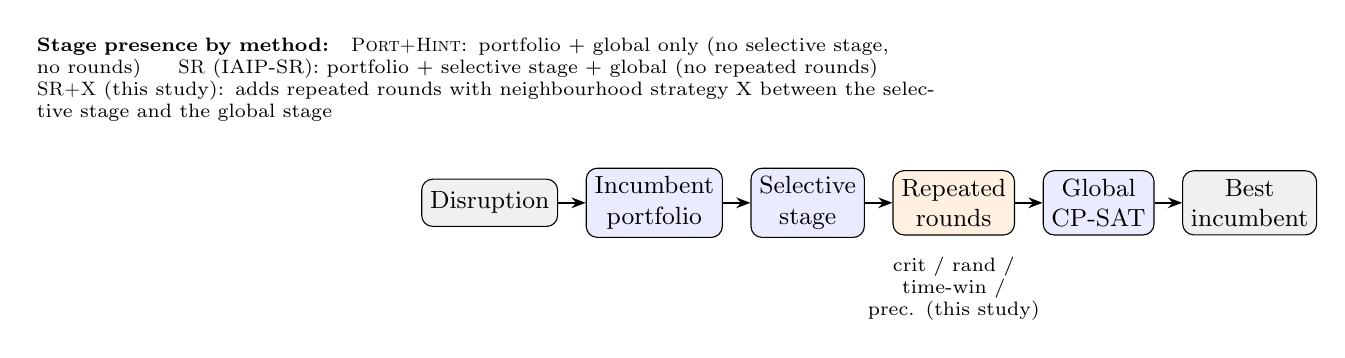
\begin{tikzpicture}[
  box/.style={draw, rounded corners, align=center, minimum height=0.6cm, font=\small, inner sep=3pt},
  arr/.style={-{Stealth[length=1.8mm]}, thick},
  node distance=0.35cm
]
\node[box, fill=gray!12] (dis) {Disruption};
\node[box, fill=blue!8, right=of dis] (port) {Incumbent\\portfolio};
\node[box, fill=blue!8, right=of port] (sel) {Selective\\stage};
\node[box, fill=orange!12, right=of sel] (rnd) {Repeated\\rounds};
\node[box, fill=blue!8, right=of rnd] (glob) {Global\\CP-SAT};
\node[box, fill=gray!12, right=of glob] (out) {Best\\incumbent};
\foreach \a/\b in {dis/port, port/sel, sel/rnd, rnd/glob, glob/out}
  \draw[arr] (\a) -- (\b);
\node[font=\scriptsize, below=0.15cm of rnd, align=center, text width=2.6cm]
  {crit / rand / time-win /\\ prec. (this study)};
\node[font=\scriptsize, above=0.6cm of dis, align=left, text width=11.5cm] (legend) {
  \textbf{Stage presence by method:}\quad
  \textsc{Port+Hint}: portfolio + global only (no selective stage, no rounds) $\quad$
  \textsc{SR} (IAIP-SR): portfolio + selective stage + global (no repeated rounds) $\quad$
  \textsc{SR+X} (this study): adds repeated rounds with neighbourhood strategy X between the selective stage and the global stage
};
\end{tikzpicture}
}
\caption{The unified pipeline and stage presence by method.}
\label{fig:framework}
\end{figure*}

\section{Repeated Restricted Reoptimization}
\label{sec:method}

After \base's single restricted stage (RQ1 isolates this stage's own value; RQ2 asks about what follows), our integration repeats the restricted solve while the local time window ($0.6B$) remains and the previous round improved the incumbent. Each round: (1) recomputes the incumbent's longest \emph{binding chains} --- the calendar-aware critical structure reused unchanged from the certificate study (below), correctly handling outages, release dates and commitments; (2) builds a neighbourhood $N$ from a round-specific targeting rule (next section); (3) solves the restricted model on $N$ (job precedence, no-overlap, outages, releases, commitments, plus the incumbent's machine order outside $N$, plus $C_{\max}\le U-1$), hinted with the incumbent; (4) accepts the result only if it strictly improves the incumbent, and (under the end-to-end protocol) stops otherwise. One monotonic deadline covers the portfolio, every round, and the final unrestricted stage; every round's restricted model always contains the current incumbent as a feasible point, so the retained objective is non-increasing by construction --- an elementary property of the acceptance rule, not a per-round guarantee: a round may still fail, time out, or return a non-improving feasible schedule, and none of this is hidden or discarded (verified below).

\section{Neighbourhood-Targeting Strategies (RQ3) and Matched External Controls}
\label{sec:lns}

Every control below (RQ3) shares the identical initial incumbent, round policy, local window, global continuation and worker count as the critical-region method, differing only in how each round's neighbourhood is chosen, so that any PI difference is attributable to neighbourhood \emph{content} rather than to a resource asymmetry.
\begin{itemize}
\item \textbf{\crit:} every operation on the incumbent's longest binding chains, expanded by 25\% breadth-first search.
\item \textbf{\rnd:} the same expansion, seeded at uniformly random operations, with $|N|$ matched exactly to \crit's neighbourhood built on the same incumbent in the same round.
\item \textbf{\tw:} $|N|$ operations consecutive in start-time order from a random index --- an external, size-matched analogue of CP-SAT's \texttt{SchedulingTime\-Window\-Neighborhood\-Generator}.
\item \textbf{\precn:} no operations freed; a uniformly random subset of machine-order precedences is released instead, matched in count to the number \crit\ releases in the same round --- an analogue of \texttt{Random\-Precedence\-Scheduling\-Neighborhood\-Generator}.
\end{itemize}
To separate the value of repetition (RQ2) from the value of targeting (RQ3), we run two protocols. \textbf{M1 (end-to-end):} each method runs until the local window or a stop-on-failure condition; round counts can differ between methods. \textbf{M2 (mechanism-isolation):} every method is fixed to exactly 6 rounds of at most 0.4\,s each, regardless of success, removing the confound that a method which more often finds nothing to improve simply finishes sooner and banks more time elsewhere.

For RQ4, \textbf{\native} is \ph\ (portfolio + hinted global CP-SAT, no repeated rounds) run with \texttt{interleave\_search} on one worker, and \ph\ at four workers is CP-SAT's default multi-worker portfolio; both were verified, from saved logs on the actual confirmatory instances (not source inspection alone), to activate all four internal scheduling LNS generators (\texttt{results/final\_icaps/solver\_logs/}), confirming both ``native LNS'' labels are accurate. CP-SAT exposes per-run subsolver filtering, but we did not use it: these configurations run the solver's ordinary default or interleaved portfolio exactly as a user would get it, where the four scheduling generators run alongside six to ten generic LNS generators, not in isolation; isolating scheduling-LNS-only behaviour is a feasible follow-up we did not run, since it answers a narrower question than any claim here makes. We compare native search only at matched worker count (1-worker-ours vs.\ 1-worker-interleaved-native; 4-worker-ours vs.\ 4-worker-native), never across worker counts; at 4 workers, U3's comparison uses $4\times$ the CPU-seconds of every 1-worker setting by design, since U3's purpose is specifically to test whether the external pipeline's advantage survives the solver's own parallel search, not to hold CPU-seconds equal (a resource-normalized, equal-core-second variant was not run; see Limitations).

\section{Correctness and the Certificate Result}
\label{sec:certificate}
\label{sec:verify}

The restriction machinery (kept-arc construction, the restricted model builder, the critical-chain computation) is reused unchanged from a prior stage, verified against two independent oracles (full enumeration and an independently-built CP-SAT model) on \OracleEnumCases\ and \OracleCpsatCases\ randomized cases with zero bound violations; for this study we additionally verified, on 250 randomized instances across all ten neighbourhood strategies with outages, release dates and commitments, that every restricted optimum lies between the full-problem optimum and the incumbent's value. A monotonic clock covers construction, every round, and the final stage; failed or non-improving rounds are recorded, not discarded; campaign resumption reproduces byte-identical output; 269 fast and 25 slow tests pass (one pre-existing, timing-sensitive integration test unrelated to this pipeline flaked once under load and passed on an immediate rerun and in isolation --- documented, not hidden, in supplementary material). A sound lower-bound \emph{certificate} for a restricted neighbourhood, verified against 5{,}500 independent oracle cases with zero violations, was decisive for only 13 of 200 restricted neighbourhoods tested; CP-SAT itself already proves the same non-improvement in a median of 21\,ms, and certificate-gated skipping, releasing, or budget allocation produced no measurable change in primal integral. We report this as a completed negative result.

\section{Experimental Methodology}

Instances are full $m\times m$ job shops ($m\in\{15,20\}$), durations uniform in $[5,50]$, ten deltas per stream drawn with weights 0.4/0.2/0.25/0.15 (arrival/cancellation/duration-change/outage). CP-SAT (OR-Tools 9.15) runs with one worker and $B=8$\,s unless stated; each process is pinned to its own physical core (four cores per process for the four-worker setting); methods of a stream run sequentially, in shuffled order, in one process.

\paragraph{Development and freeze.} All method and control design used development streams (seeds 301--310) across three rounds, each round's question and decision rule written down before it ran; the final configuration, comparator set, and GO/CONDITIONAL-GO/NO-GO criteria were frozen (file hash checked before any held-out run) \emph{before} any run on the confirmatory streams.

\paragraph{Confirmation.} The held-out data are stream seeds 1101--1120 (40 streams, confirmed unused anywhere in this project's history, scanned explicitly), solver seeds 0--4. Forty streams means 2 instance sizes $\times$ 20 distinct seed values, not 40 independent seed values; seed numbers are shared across sizes, which we verified does not create a non-independence problem, since every analysis groups by the full size-and-seed stream identifier, never the bare seed number, and the two sizes produce genuinely different random draws from the first size-dependent step onward. Nine settings run in a fixed order: \textbf{U1} primary (8\,s, 1 worker, all seven methods); \textbf{U2} mechanism-isolation (M2, four strategies); \textbf{U3} four workers (20 streams); \textbf{U4}--\textbf{U9} secondary (2\,s; 30\,s; arrival-only; outage-only; high severity; 34 published job-shop bases --- Taillard, DMU, SWV, YN --- one stream per base, the base instance as the unit). The unit of inference is the stream (or base instance for U9); PI is averaged over steps 1--10 and solver seeds within a unit before any comparison; tests are the exact sign test over units with Holm correction within each setting's declared family, plus a stream-clustered bootstrap 95\% CI (10{,}000 resamples). An equivalence margin of $\pm10\%$ of the comparator's mean PI was fixed in advance for the critical-vs-time-window question, informed by a development power calculation showing differences below roughly 15--17\% of mean PI would not reliably reach significance at this sample size.

\paragraph{Criteria (fixed before the run).} C1: \crit\ beats \base\ by $\ge5\%$, CI upper $<0$, Holm $p<0.05$. C2: beats \rnd, CI upper $<0$. C3: vs.\ \tw, classified superior/inferior/equivalent/inconclusive by the sign/significance/equivalence rule above. C4: beats \precn. C5: beats \native\ (1 worker). C6: beats \ph\ at 4 workers. \textbf{STRONG GO} requires C1--C6 all favourable; \textbf{CONDITIONAL GO} requires C1 and validity but allows C3 non-superior or C6 to fail, with no claim of superior critical-region search made in that case; \textbf{NO-GO} if C1 fails or C3 is inferior.

\paragraph{Independent re-verification.} All 60{,}720 confirmatory runs were re-checked by a second analysis pipeline sharing no code with the one that produced the reported statistics (its own feasibility checker, PI integrator, sign test, Holm correction and bootstrap). Every one of the 33 reported confirmatory comparisons reproduced to floating-point rounding (relative-difference error $<1.2\times10^{-16}$), with identical win/loss counts and Holm-adjusted $p$-values in every case (\texttt{re\-sults/\-fi\-nal\_i\-caps/\-ver\-i\-fied\_met\-rics.json}).

\begin{table*}[t]
\centering
\small
\setlength{\tabcolsep}{4pt}
\begin{tabular}{lrrrrrrr}
\toprule
Setting & $n$ & \crit & \base & \ph & vs.\ \base & vs.\ \tw & vs.\ \native/\ph(4w) \\
\midrule
U1: 8\,s, 1w & \UOneN & \UOneMeanBTwocrit & \UOneMeanBZeroiaip & \UOneMeanBSixporthint &
  $\UOneBTwocritVsBZeroiaipSign\UOneBTwocritVsBZeroiaipRel$\% (\UOneBTwocritVsBZeroiaipWL) &
  $\UOneBTwocritVsBThreetimewinSign\UOneBTwocritVsBThreetimewinRel$\% (\UOneBTwocritVsBThreetimewinWL) &
  $\UOneBTwocritVsBFivenativeOnewSign\UOneBTwocritVsBFivenativeOnewRel$\% (\UOneBTwocritVsBFivenativeOnewWL) \\
U3: 8\,s, 4w & \UThreeN & \UThreeMeanBTwocrit & \UThreeMeanBZeroiaip & \UThreeMeanBSixporthint &
  $\UThreeBTwocritVsBZeroiaipSign\UThreeBTwocritVsBZeroiaipRel$\% (\UThreeBTwocritVsBZeroiaipWL) &
  $\UThreeBTwocritVsBThreetimewinSign\UThreeBTwocritVsBThreetimewinRel$\% (\UThreeBTwocritVsBThreetimewinWL) &
  $\UThreeBTwocritVsBSixporthintSign\UThreeBTwocritVsBSixporthintRel$\% (\UThreeBTwocritVsBSixporthintWL) \\
U4: 2\,s, 1w & \UFourN & \UFourMeanBTwocrit & \UFourMeanBZeroiaip & \UFourMeanBSixporthint &
  $\UFourBTwocritVsBZeroiaipSign\UFourBTwocritVsBZeroiaipRel$\% (\UFourBTwocritVsBZeroiaipWL) &
  $\UFourBTwocritVsBThreetimewinSign\UFourBTwocritVsBThreetimewinRel$\% (\UFourBTwocritVsBThreetimewinWL) & -- \\
U5: 30\,s, 1w & \UFiveN & \UFiveMeanBTwocrit & \UFiveMeanBZeroiaip & \UFiveMeanBSixporthint &
  $\UFiveBTwocritVsBZeroiaipSign\UFiveBTwocritVsBZeroiaipRel$\% (\UFiveBTwocritVsBZeroiaipWL) &
  $\UFiveBTwocritVsBThreetimewinSign\UFiveBTwocritVsBThreetimewinRel$\% (\UFiveBTwocritVsBThreetimewinWL) & -- \\
U6: arrival-only & \USixN & \USixMeanBTwocrit & \USixMeanBZeroiaip & \USixMeanBSixporthint &
  $\USixBTwocritVsBZeroiaipSign\USixBTwocritVsBZeroiaipRel$\% (\USixBTwocritVsBZeroiaipWL) &
  $\USixBTwocritVsBThreetimewinSign\USixBTwocritVsBThreetimewinRel$\% (\USixBTwocritVsBThreetimewinWL) & -- \\
U7: outage-only & \USevenN & \USevenMeanBTwocrit & \USevenMeanBZeroiaip & \USevenMeanBSixporthint &
  $\USevenBTwocritVsBZeroiaipSign\USevenBTwocritVsBZeroiaipRel$\% (\USevenBTwocritVsBZeroiaipWL) &
  $\USevenBTwocritVsBThreetimewinSign\USevenBTwocritVsBThreetimewinRel$\% (\USevenBTwocritVsBThreetimewinWL) & -- \\
U8: high severity & \UEightN & \UEightMeanBTwocrit & \UEightMeanBZeroiaip & \UEightMeanBSixporthint &
  $\UEightBTwocritVsBZeroiaipSign\UEightBTwocritVsBZeroiaipRel$\% (\UEightBTwocritVsBZeroiaipWL) &
  $\UEightBTwocritVsBThreetimewinSign\UEightBTwocritVsBThreetimewinRel$\% (\UEightBTwocritVsBThreetimewinWL) & -- \\
U9: 34 bases & \UNineN & \UNineMeanBTwocrit & \UNineMeanBZeroiaip & \UNineMeanBSixporthint &
  $\UNineBTwocritVsBZeroiaipSign\UNineBTwocritVsBZeroiaipRel$\% (\UNineBTwocritVsBZeroiaipWL) &
  $\UNineBTwocritVsBThreetimewinSign\UNineBTwocritVsBThreetimewinRel$\% (\UNineBTwocritVsBThreetimewinWL) & -- \\
\bottomrule
\end{tabular}
\caption{Held-out confirmation (stream seeds 1101--1120, solver seeds 0--4 unless stated; U5 uses seeds 0--2). Mean PI per method ($n$: streams, or base instances for U9); relative PI difference and streams won/lost (\crit\ vs.\ each comparator).}
\label{tab:conf}
\end{table*}

\section{Results}
\label{sec:results}

All \UOneRecords{} U1 and 60{,}720 total confirmatory runs returned a validated schedule (0 invalid, 0 unsolved); Table~\ref{tab:conf} and Figure~\ref{fig:traj} summarize the confirmatory evidence.

\paragraph{RQ1/RQ2: repeated rounds beat the one-round pipeline; unstructured repetition alone does not.} \crit\ reduces mean PI by \UOneBTwocritVsBZeroiaipRel\% relative to \base{} in U1 (\UOneBTwocritVsBZeroiaipWL, CI $\UOneBTwocritVsBZeroiaipCI$, Holm $p=\UOneBTwocritVsBZeroiaipHolm$) --- \textbf{C1 holds.} But \rnd{} itself is \emph{not} significantly better than \base{} ($\UOneBOnerandomVsBZeroiaipRel$\%, \UOneBOnerandomVsBZeroiaipWL, Holm $p=\UOneBOnerandomVsBZeroiaipHolm$): repeating the restricted stage with an unstructured neighbourhood adds almost nothing by itself. Targeted repetition beats unstructured repetition: \crit\ vs.\ \rnd{} is $\UOneBTwocritVsBOnerandomRel$\% (\UOneBTwocritVsBOnerandomWL, Holm $p=\UOneBTwocritVsBOnerandomHolm$), and \crit\ vs.\ \precn{} (random-precedence relaxation) is $\UOneBTwocritVsBFourprecRel$\% (\UOneBTwocritVsBFourprecWL) --- \textbf{C2 and C4 hold.}

\paragraph{RQ3: does critical targeting beat time-window targeting?} In U1, \crit\ vs.\ \tw{} is $\UOneBTwocritVsBThreetimewinRel$\% (\UOneBTwocritVsBThreetimewinWL, Holm $p=\UOneBTwocritVsBThreetimewinHolm$) --- not significant. An initial by-disruption-type breakdown of this same (end-to-end) comparison suggested an exception after arrivals (\USixBTwocritVsBThreetimewinSign\USixBTwocritVsBThreetimewinRel\%, \USixBTwocritVsBThreetimewinWL, Holm $p=\USixBTwocritVsBThreetimewinHolm$, U6). We investigated this further (the next section) rather than reporting it as a confirmed exception, and found it does not survive matched-round accounting: \textbf{C3 is inconclusive overall, and the apparent arrival exception does not hold once round count is controlled for}.

\paragraph{RQ4: native solver search.} \crit\ vs.\ \native{} (1-worker, confirmed from logs to run all four scheduling LNS generators on one thread): $\UOneBTwocritVsBFivenativeOnewRel$\% (\UOneBTwocritVsBFivenativeOnewWL, Holm $p=\UOneBTwocritVsBFivenativeOnewHolm$) --- \textbf{C5 holds.} At four workers (U3, confirmed from logs to run the same four generators alongside three more), \crit\ vs.\ \ph{} is $\UThreeBTwocritVsBSixporthintRel$\% (\UThreeBTwocritVsBSixporthintWL, Holm $p=\UThreeBTwocritVsBSixporthintHolm$) --- not significant; \crit\ vs.\ \base{} at four workers is $\UThreeBTwocritVsBZeroiaipRel$\% ($\UThreeBTwocritVsBZeroiaipWL$), also not significant. \textbf{C6 fails}: with CP-SAT's own multi-worker scheduling LNS active, none of \base, \crit{} or \tw{} is distinguishable from the others.

\paragraph{RQ6: robustness.} The advantage over \base{} holds in every secondary setting except U4 (2\,s: $\UFourBTwocritVsBZeroiaipRel$\%, Holm $p=\UFourBTwocritVsBZeroiaipHolm$) and is strongest on published bases ($\UNineBTwocritVsBZeroiaipRel$\%, U9).

\begin{figure}[t]
\centering
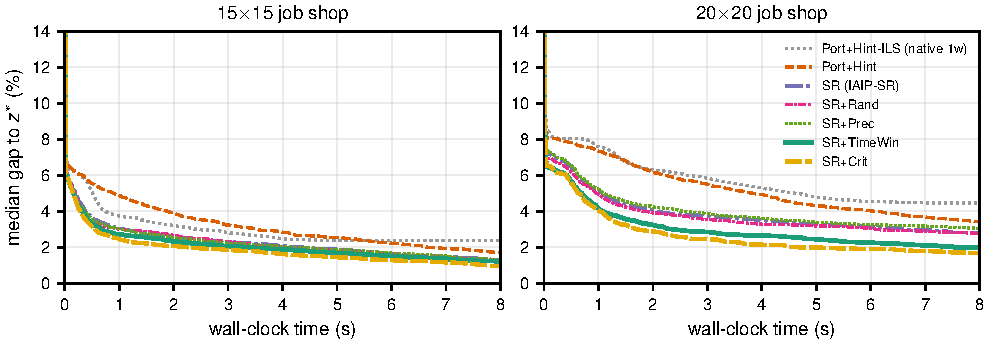
\includegraphics[width=\linewidth]{figures/trajectories.pdf}
\caption{Median gap to $z^*$ over time, U1 confirmatory streams (1{,}000 instance-step-seed combinations per size per method). Real archived trajectories, not illustrative curves. At $B=8$\,s, \crit{} and \tw{} reach \FigTwoOneFiveCritAt\% / \FigTwoOneFiveTwAt\% ($15{\times}15$) and \FigTwoTwoZeroCritAt\% / \FigTwoTwoZeroTwAt\% ($20{\times}20$) median gap, both well ahead of \base{} (\FigTwoOneFiveSrAt\% / \FigTwoTwoZeroSrAt\%).}
\label{fig:traj}
\end{figure}

\section{Resolving the Disruption-Type Question by Reanalysis}
\label{sec:timewindow}

No new experiments were run for this section; it reanalyses already-archived U1/U2 raw trajectories, which can answer the question directly. Breaking out U2's existing mechanism-isolation (fixed 6-round) comparison by disruption type (exploratory grouping, not in the pre-registered family, no multiplicity correction) gives, for every type including arrivals, a result with the \emph{opposite} sign from U6's end-to-end comparison: critical targeting is **worse** than time-window targeting once round count is fixed (arrival $\MechTwoArrivalRel$\%, \MechTwoArrivalWL, crit worse; cancellation $\MechTwoCancellationRel$\%, \MechTwoCancellationWL; duration change $\MechTwoDurationRel$\%, \MechTwoDurationWL; outage $\MechTwoOutageRel$\%, \MechTwoOutageWL; all $n\approx$30--40 streams).

The mechanism: under the end-to-end protocol, critical-region rounds complete systematically more rounds per instance than time-window rounds in every disruption type (U1: arrival \RoundsUOneArrivalCrit{} vs.\ \RoundsUOneArrivalTw; cancellation \RoundsUOneCancelCrit{} vs.\ \RoundsUOneCancelTw; duration change \RoundsUOneDurationCrit{} vs.\ \RoundsUOneDurationTw; outage \RoundsUOneOutageCrit{} vs.\ \RoundsUOneOutageTw), because critical-region rounds succeed more often per attempt and the stop-on-fail rule lets a method continue only after success. More attempted rounds mean more chances to improve, independent of whether the neighbourhood content is actually better --- exactly the confound the fixed-round protocol is designed to remove. \textbf{We therefore do not claim critical targeting is better suited to any disruption type}; the apparent arrival exception is an artifact of unequal round counts, not of neighbourhood content, and this supersedes our own earlier reading of the same end-to-end data.

A further reanalysis of U2's round-level metadata shows neighbourhood \emph{size} is matched almost exactly between critical and time-window rounds (\MTwoRoundCritN{} vs.\ \MTwoRoundTwN{} operations) but the resulting restricted subproblem's \emph{difficulty} is not: time-window rounds take \MTwoRoundTwVsCritPct\% longer to resolve on average (\MTwoRoundTwSolverS\,s vs.\ \MTwoRoundCritSolverS\,s) and more often exhaust their 0.4\,s cap without a definitive status (\MTwoRoundTwFeas\ vs.\ \MTwoRoundCritFeas\ rounds), while critical-region rounds more often resolve quickly to a proof of no improvement (\MTwoRoundCritInfeas\ vs.\ \MTwoRoundTwInfeas). Equal neighbourhood size does not imply equal search complexity, and this asymmetry is a candidate explanation for why a size-matched time-window neighbourhood is, overall, at least as effective as the incumbent's critical region despite containing far fewer operations that are actually on a critical chain.

\section{Discussion and Limitations}
\label{sec:discussion}

Per our pre-registered classification, this is a \textbf{CONDITIONAL GO}: C1, C2, C4 and C5 hold reproducibly; C3 is not established as superior (and, after reanalysis, not even conditionally so after arrivals); C6 fails outright. We do \emph{not} claim critical-region search is a superior targeting mechanism. The defensible claim is narrower: (1) repeating the restricted stage with a \emph{recomputed}, spatially-coherent neighbourhood substantially improves anytime quality over a single stage, but only when the neighbourhood is coherent, not chosen uniformly at random or as random precedence relaxations; (2) which coherent region is used --- the critical chain or a time window of matched size --- does not reliably matter, and a reanalysis that removes a round-count confound shows time-window is, if anything, the slightly better choice in every disruption type tested; (3) this entire family of findings is specific to a single CP-SAT worker and does not survive the solver's own multi-worker scheduling search, which on these instances is already strong enough that none of the external neighbourhood strategies adds anything beyond it.

Instances are synthetic full job shops from one generator; development and held-out streams share that generator. $z^*$ is the best value found in each setting, not a proven optimum. Only makespan is optimized; stability is not controlled. The C3 equivalence classification depends on a pre-specified $\pm10\%$ margin and a development-derived power estimate; non-significance under that margin is absence of demonstrated superiority, not proof of equivalence. CP-SAT's internal LNS generator selection is solver-version-specific; a different OR-Tools release could show different four-worker behaviour. U3's four-worker comparison uses $4\times$ the CPU-seconds of the one-worker settings by design (matched wall-clock, not matched core-seconds); a resource-normalized variant was not run and is left for future work, as is a scheduling-LNS-only native baseline (feasible via \texttt{extra\_subsolvers} with a retained core-search subsolver, not attempted here). The full texts of \citet{sun2026} and \citet{linyang2026} remain inaccessible to us despite a renewed, documented attempt through legitimate routes.

\section{Conclusion}

Across a frozen, independently-reproduced confirmatory study, retaining a feasible incumbent and repeating a restricted CP-SAT stage with a recomputed, spatially-coherent neighbourhood reliably improves an anytime rescheduling pipeline over a single restricted stage, over unstructured repetition, and over the installed solver's single-thread scheduling search. Whether that coherent region should be the schedule's critical chain specifically, rather than a comparably simple time window, is not established by this evidence in any disruption type we tested once a round-count confound is removed; and the entire advantage over native search disappears once the solver is allowed to use its own multiple workers. We report the positive and the negative findings together, and the reanalysis that narrowed our own initial reading of the data, as the more defensible outcome of this investigation.

\bibliography{references}

\end{document}
